\problemname{Coast Length}
The island municipality of Soteholm is required to write a plan of action for their work with emission of greenhouse gases. They realize that a natural first step is to decide whether they are for or against global warming.
For this purpose they have read the IPCC report on climate change and found out that the largest effect on their
municipality could be the rising sea level.

The residents of Soteholm value their coast highly and therefore want to maximize its total length. For them
to be able to make an informed decision on their position in the issue of global warming, you have to help them
find out whether their coastal line will shrink or expand if the sea level rises. From height maps they have figured
out what parts of their islands will be covered by water, under the different scenarios described in the IPCC report,
but they need your help to calculate the length of the coastal lines.

\section*{Task}
You will be given a map of Soteholm as an $N \times M$ grid. Each square in the grid has a side length of $1$ km and is
either water or land. Your goal is to compute the total length of sea coast of all islands. Sea coast is all borders
between land and sea, and sea is any water connected to an edge of the map only through water. Two squares are
connected if they share an edge. You may assume that the map is surrounded by sea. Lakes and islands in lakes
are not contributing to the sea coast.

\begin{figure}[h]
    \centering
    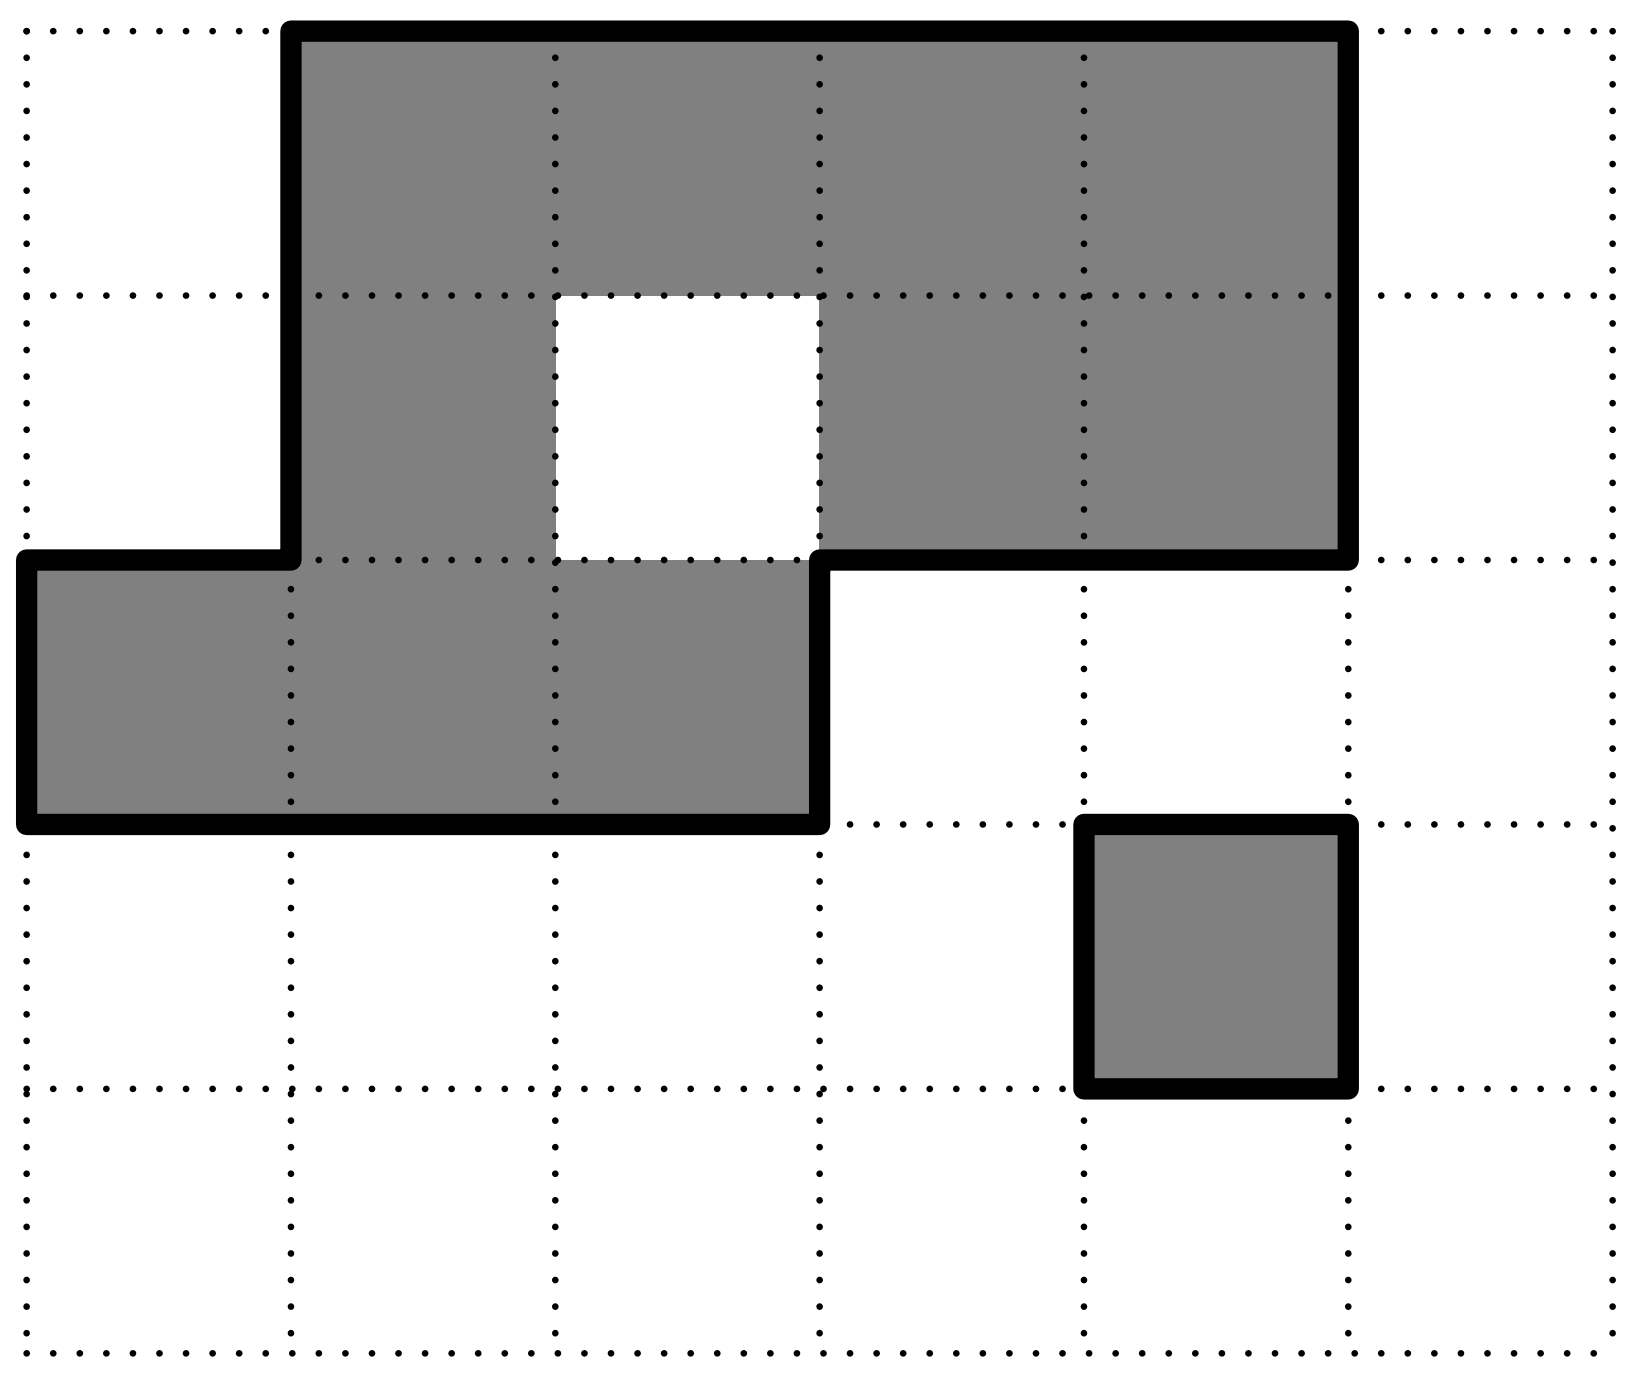
\includegraphics[width=0.3\textwidth]{fig.png}
    \caption{Gray squares are land and white squares are water. The thick black line is the sea coast. This example corresponds to Sample Input 1.}
\end{figure}

\section*{Input}
The first line of the input contains two space separated integers $N$ and $M$ where $1 \le N, M \le 1000$.
The following $N$ lines each contain a string of length $M$ consisting of only zeros and ones.
Zero means water and one means land.

\section*{Output}
Output one line with one integer, the total length of the coast in km.
